% ------------------------------------------------------------------------------
% Your readers must be able to understand at a glance which data set belongs to which research question or hypothesis.
% - Describe your data objectively
% - Use graphs and tables to illustrate your data.
% - Refer to your research question with each result
% - Rank your results in order of importance
% - Confirm or reject your hypotheses
% ------------------------------------------------------------------------------

\opt{never}{\addbibresource{03-tail/bibliography.bib}} % to make citation found in most IDE

\chapter{Validation}
\label{chap:validation}

% -- Your text goes here --
This chapter presents the tests carried out and their results to prove that the reference architecture works in its entirety. The notion of cost at \gls{cloud_infrastructure} level is also addressed. 

\minitoc
\newpage

% -----------------------------------------------------------------------------
\section{Project configuration}

% -- Your text goes here --
Before pushing this reference architecture into a new GitHub repository, a few project configurations have been made. Firstly, it is essential to add the GitHub Actions user as a trusted identity so that \gls{aws} can grant him access to its resources. In the \gls{aws} account on which the infrastructure is deployed, the GitHub identity provider is specified (figure \ref{fig:1_Identity_provider}).
\begin{center}
    \begingroup
    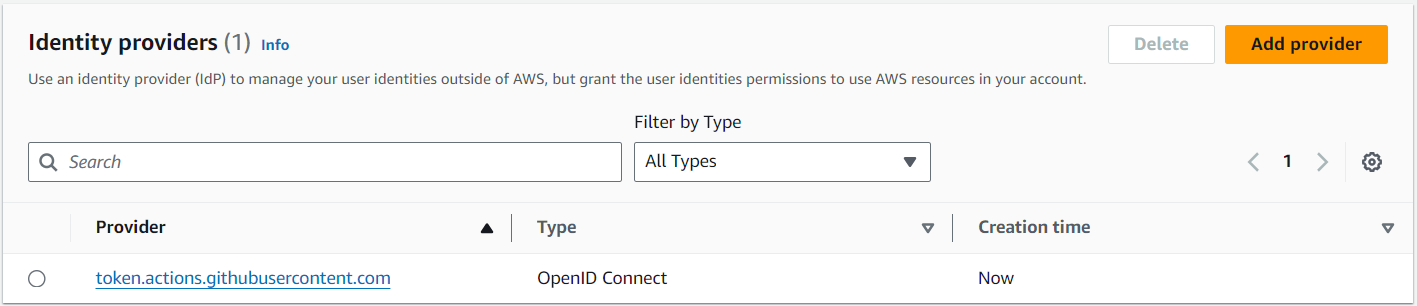
\includegraphics[width=1\columnwidth]{validation/1_Identity_provider.png}
    \captionof{figure}{GitHub identity provider}
    \label{fig:1_Identity_provider}
    \endgroup
\end{center}
An IAM role has been set up to authorise only the project's GitHub repository to access resources. A policy is linked to limit the actions allowed on the resources (figure \ref{fig:2_OIDCRole}).
\begin{center}
    \begingroup
    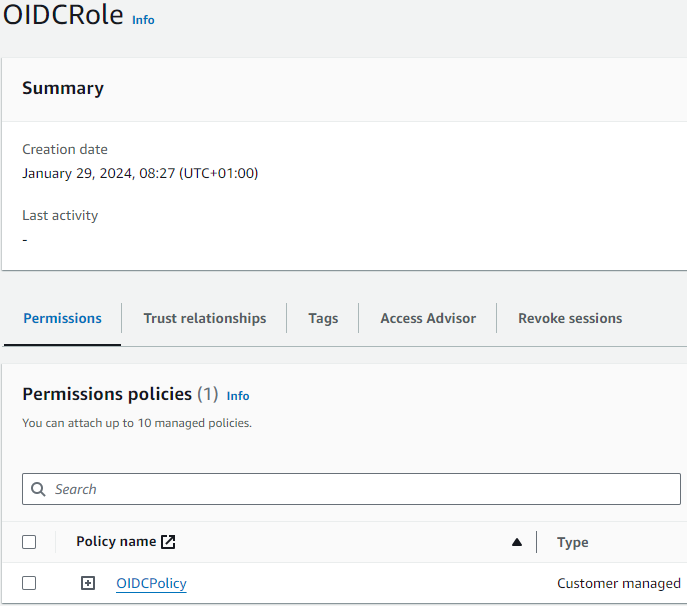
\includegraphics[width=.8\columnwidth]{validation/2_OIDCRole.png}
    \captionof{figure}{IAM OIDC role}
    \label{fig:2_OIDCRole}
    \endgroup
\end{center}
The secret and visible variables that need to be configured have been added to the GitHub repository (figures \ref{fig:3_SecretVar_GitHub} and \ref{fig:3_Var_GitHub}).
\begin{center}
    \begingroup
    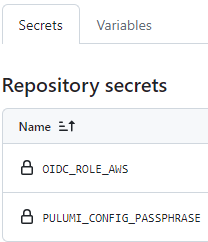
\includegraphics[width=.25\columnwidth]{validation/3_SecretVar_GitHub.png}
    \captionof{figure}{GitHub secret variables}
    \label{fig:3_SecretVar_GitHub}
    \endgroup
\end{center}
\begin{center}
    \begingroup
    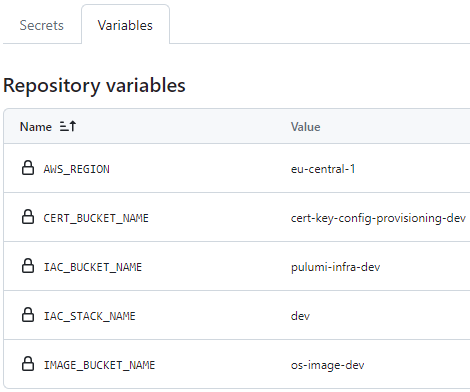
\includegraphics[width=.5\columnwidth]{validation/3_Var_GitHub.png}
    \captionof{figure}{GitHub visible variables}
    \label{fig:3_Var_GitHub}
    \endgroup
\end{center}
The configuration file for the Pulumi tool was configured by specifying the \gls{aws} account ID and the region (figure \ref{fig:4_Set_Pulumi_Stack}).
\begin{center}
    \begingroup
    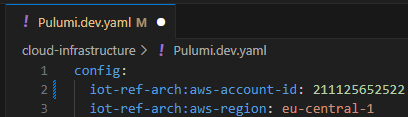
\includegraphics[width=.55\columnwidth]{validation/4_Set_Pulumi_Stack.png}
    \captionof{figure}{Pulumi configuration file (development environment)}
    \label{fig:4_Set_Pulumi_Stack}
    \endgroup
\end{center}
Finally, the serial numbers of the devices authorised to be provisioned have been listed. In this case, only a Raspberry Pi 4 is authorised (figure \ref{fig:5_Set_Allowlist}).
\begin{center}
    \begingroup
    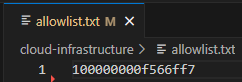
\includegraphics[width=.3\columnwidth]{validation/5_Set_Allowlist.png}
    \captionof{figure}{Embedded systems allowlist}
    \label{fig:5_Set_Allowlist}
    \endgroup
\end{center}

\section{\texorpdfstring{\acrshort{ci}/\acrshort{cd}}{} pipeline}

% -- Your text goes here --
After the previous configuration, the project was pushed into the GitHub repository. The \acrshort{ci}/\acrshort{cd} pipeline started automatically, beginning with the deployment of the \gls{cloud_infrastructure}. All tasks were completed successfully. The different times for each workflow can be seen on the right-hand side of figure \ref{fig:6_Workflows}. Total process time is just over 10 minutes.
\begin{center}
    \begingroup
    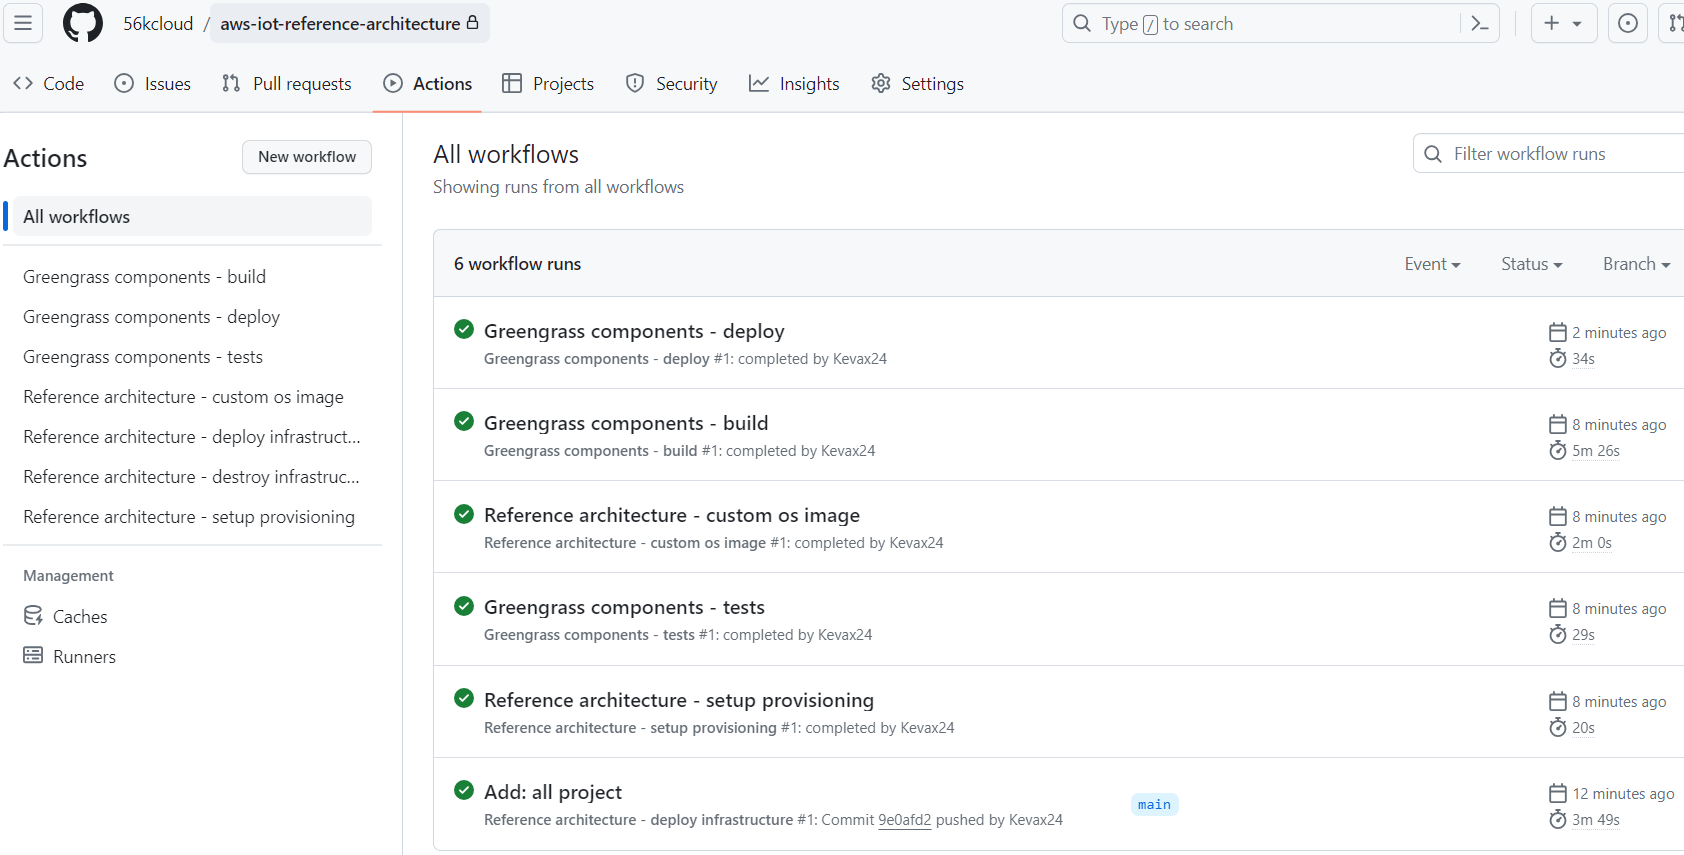
\includegraphics[width=1\columnwidth]{validation/6_Workflows.png}
    \captionof{figure}{Successful workflows}
    \label{fig:6_Workflows}
    \endgroup
\end{center}
The \gls{cloud_infrastructure} has been deployed on the development account specified and in the \textit{eu-central-1} region. The configuration for the provisioning of the embedded systems was carried out correctly with the creation of the \acrshort{os} image. The base image used is \textit{Raspberry Pi \acrshort{os} Lite} based on the Debian distribution.

At the same time, the applications were tested, including the led application, the button application and the certificate rotation application. Five Greengrass components were created and published in \gls{aws}. These components were also deployed.

\section{\texorpdfstring{\Gls{cloud_infrastructure}}{} deployment}

% -- Your text goes here --
All the resources described in Pulumi have been created correctly. In this sequel, they are not all mentioned and presented in images due to the sheer number of resources. An example is shown in figure \ref{fig:10_Infra_S3} where the S3 buckets have been created. There is the storage space for the state of the infrastructure, another for the provisioning configuration and finally one where the \acrshort{os} image is stored.
\begin{center}
    \begingroup
    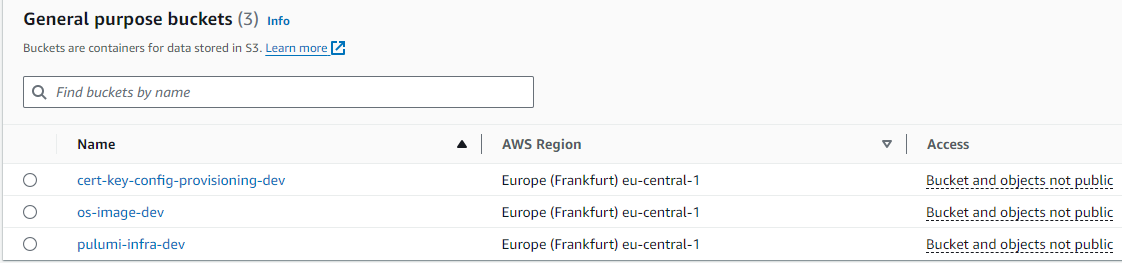
\includegraphics[width=1\columnwidth]{validation/10_Infra_S3.png}
    \captionof{figure}{S3 buckets}
    \label{fig:10_Infra_S3}
    \endgroup
\end{center}
The \acrshort{iot} device group has been created under the \textit{GreengrassGroup} name. Two policies were created for \gls{provisioning} and for interactions once provisioned (figure \ref{fig:10_Infra_IoT_Policies}). The claim certificate has also been prepared and linked to the \gls{provisioning} policy.
\begin{center}
    \begingroup
    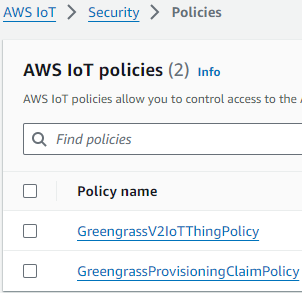
\includegraphics[width=.3\columnwidth]{validation/10_Infra_IoT_Policies.png}
    \captionof{figure}{\acrshort{iot} policies}
    \label{fig:10_Infra_IoT_Policies}
    \endgroup
\end{center}
The Greengrass components have been successfully published (figure \ref{fig:10_Infra_IoT_Components}). Docker images of the applications are also available in the Amazon \acrshort{ecr} service.
\begin{center}
    \begingroup
    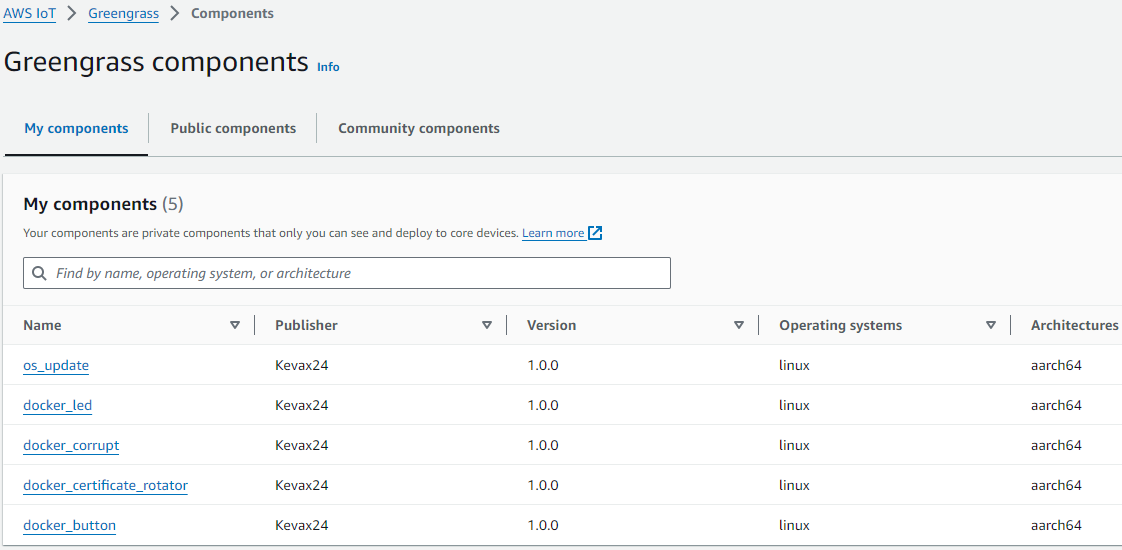
\includegraphics[width=1\columnwidth]{validation/10_Infra_IoT_Components.png}
    \captionof{figure}{Greengrass components}
    \label{fig:10_Infra_IoT_Components}
    \endgroup
\end{center}
A deployment service is ready to deploy applications as soon as devices are provisioned. It targets the group created (figure \ref{fig:10_Infra_IoT_Deployment}).
\begin{center}
    \begingroup
    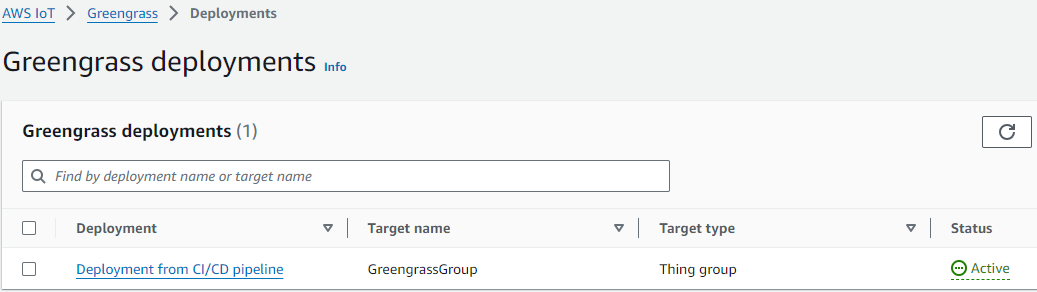
\includegraphics[width=1\columnwidth]{validation/10_Infra_IoT_Deployment.png}
    \captionof{figure}{\gls{aws} \acrshort{iot} Greengrass Deployment}
    \label{fig:10_Infra_IoT_Deployment}
    \endgroup
\end{center}

\section{\texorpdfstring{\Gls{provisioning}}{} a Raspberry Pi 4}

% -- Your text goes here --
The integration of an \acrshort{iot} device was a success. A Raspberry Pi 4 was provisioned. The \acrshort{os} image was first downloaded from the S3 bucket. It was then flashed into an SD card (figure \ref{fig:7_Flashing_SDCard}).
\begin{center}
    \begingroup
    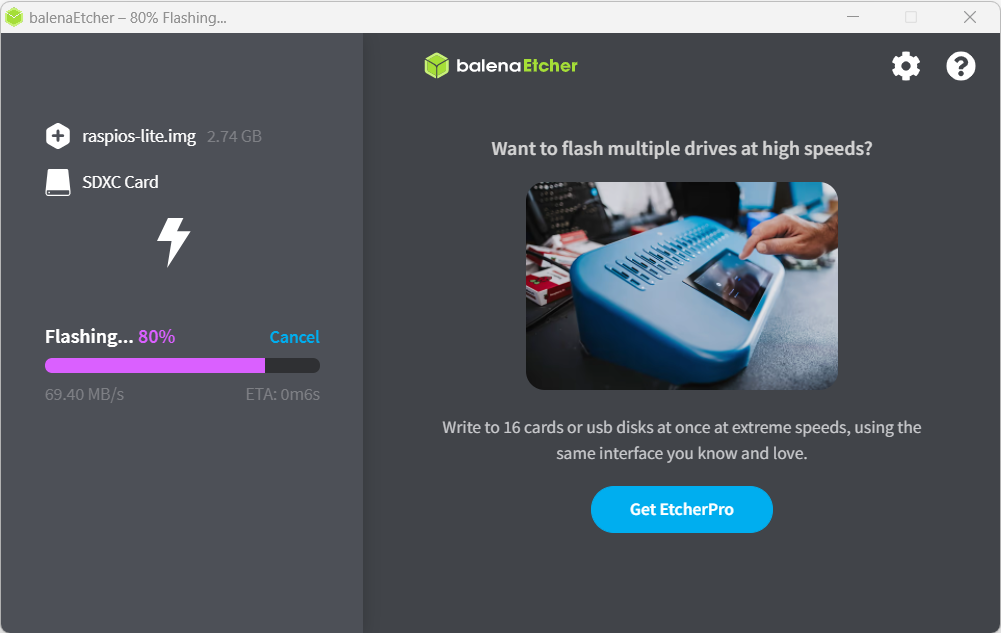
\includegraphics[width=.9\columnwidth]{validation/7_Flashing_SDCard.png}
    \captionof{figure}{\acrshort{os} image flashing}
    \label{fig:7_Flashing_SDCard}
    \endgroup
\end{center}
The Raspberry Pi 4 was then powered up and booted for the first time. All the software was installed and \gls{provisioning} was successfully completed (figure \ref{fig:8_Provisioning_Done}).
\begin{center}
    \begingroup
    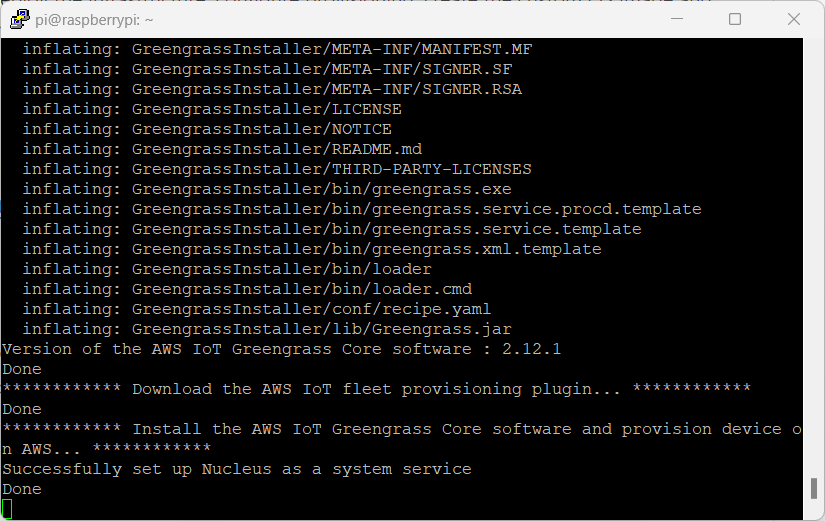
\includegraphics[width=.9\columnwidth]{validation/8_Provisioning_Done.png}
    \captionof{figure}{End of \gls{provisioning} on the device}
    \label{fig:8_Provisioning_Done}
    \endgroup
\end{center}
\Gls{provisioning} is confirmed in figure \ref{fig:8_Provisioned_AWS}. \gls{aws} has created a digital twin of this device on the \gls{aws} \acrshort{iot} service. The name corresponds to its serial number. It is linked to the group created earlier. A unique X.509 certificate has been provided.
\begin{center}
    \begingroup
    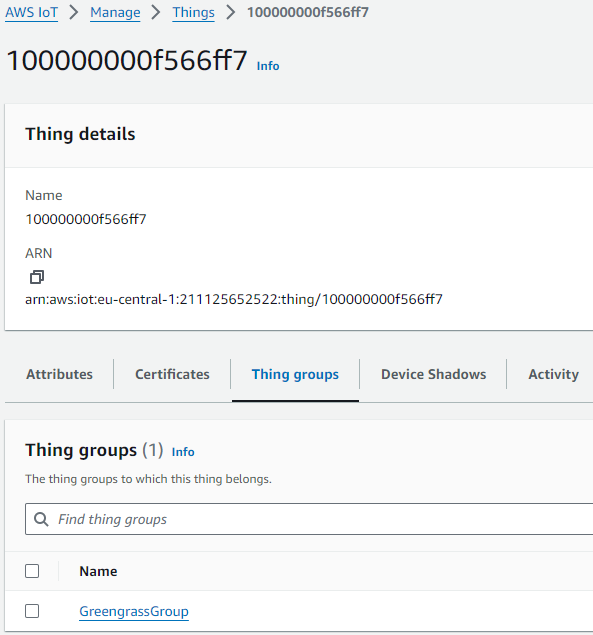
\includegraphics[width=.6\columnwidth]{validation/8_Provisioned_AWS.png}
    \captionof{figure}{Confirmed \gls{provisioning} on \gls{aws}}
    \label{fig:8_Provisioned_AWS}
    \endgroup
\end{center}

\subsection{Adding a second Raspberry Pi 4}

\section{Applications}

% -- Your text goes here --
All the applications were deployed on the Raspberry Pi 4. As soon as it was provisioned, the deployment started. This can be seen in figure \ref{fig:9_Deployment_InProgress}.
\begin{center}
    \begingroup
    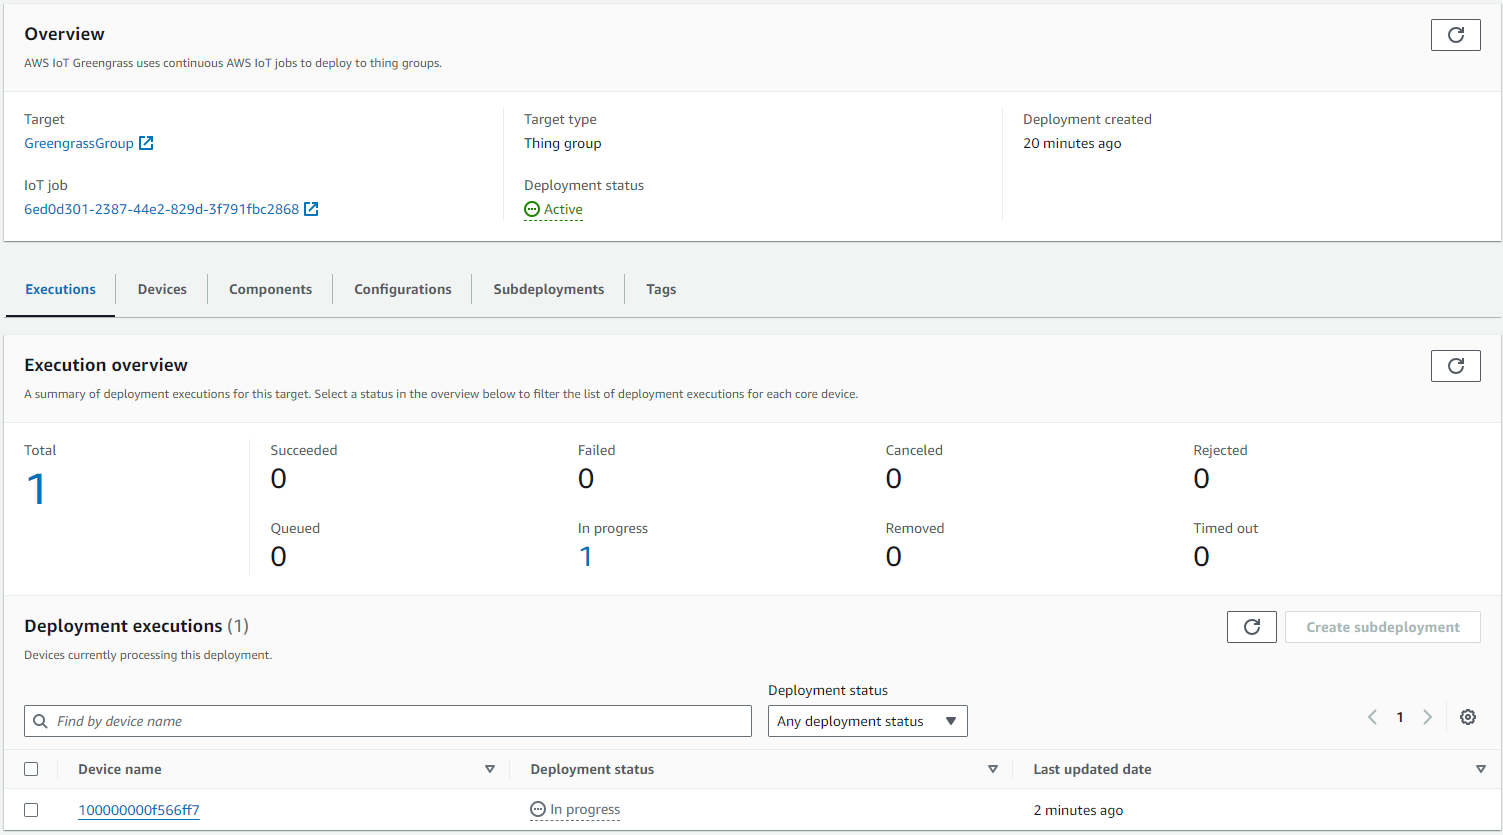
\includegraphics[width=1\columnwidth]{validation/9_Deployment_InProgress.png}
    \captionof{figure}{Deployment of Greengrass components in progress}
    \label{fig:9_Deployment_InProgress}
    \endgroup
\end{center}
Deployment took just a few minutes. The Greengrass components acting as intermediaries for the applications can be seen in figure \ref{fig:11_Components_Running}. The dependencies are also installed in addition to the Greengrass nucleus \textit{aws.greengrass.Nucleus}.
\begin{center}
    \begingroup
    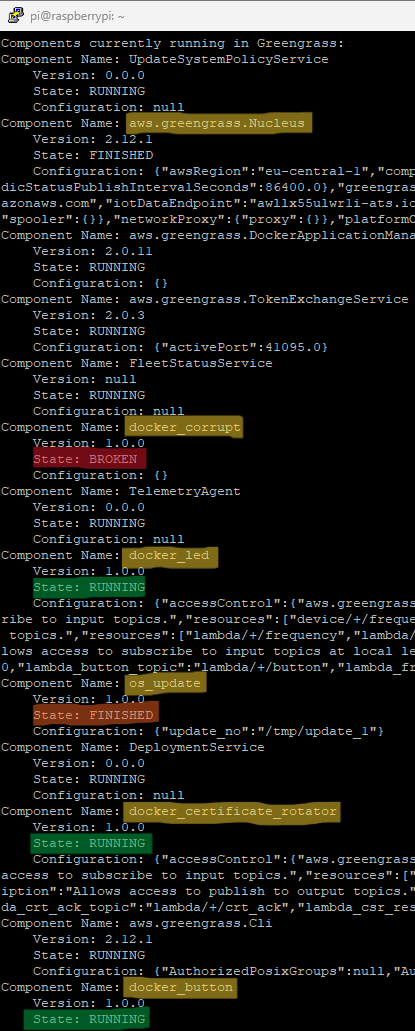
\includegraphics[width=.5\columnwidth]{validation/11_Components_Running.png}
    \captionof{figure}{Greengrass components deployed}
    \label{fig:11_Components_Running}
    \endgroup
\end{center}
It is possible to see an overview of the Raspberry Pi 4 on \gls{aws} as shown in figure \ref{fig:13_DeviceHealth}. Its state of health is poor because a component failed when it was launched. In fact, the corrupted component was unable to start up correctly and was interrupted. The other components are in a state of execution or completion.
\begin{center}
    \begingroup
    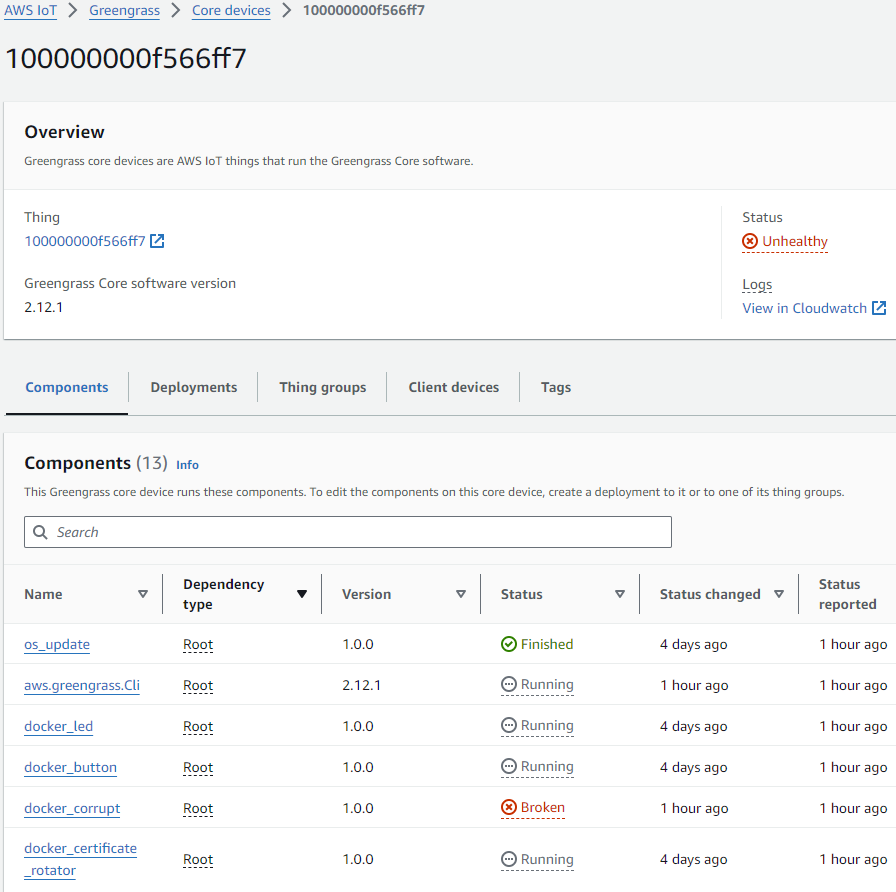
\includegraphics[width=1\columnwidth]{validation/13_DeviceHealth.png}
    \captionof{figure}{Overview of the Raspberry Pi 4 from \gls{aws}}
    \label{fig:13_DeviceHealth}
    \endgroup
\end{center}

\subsection{Applications interaction}
The applications were then tested. The first was the led application. The \gls{aws} web interface was used to send \acrshort{mqtt} messages and view the data received. A message is sent to the Raspberry Pi 4 to change its led blinking frequency. A response was sent back to \gls{aws} \acrshort{iot} in another field including the new frequency. A proof can be found in figure \ref{fig:12_FrequencyChange}.
\begin{center}
    \begingroup
    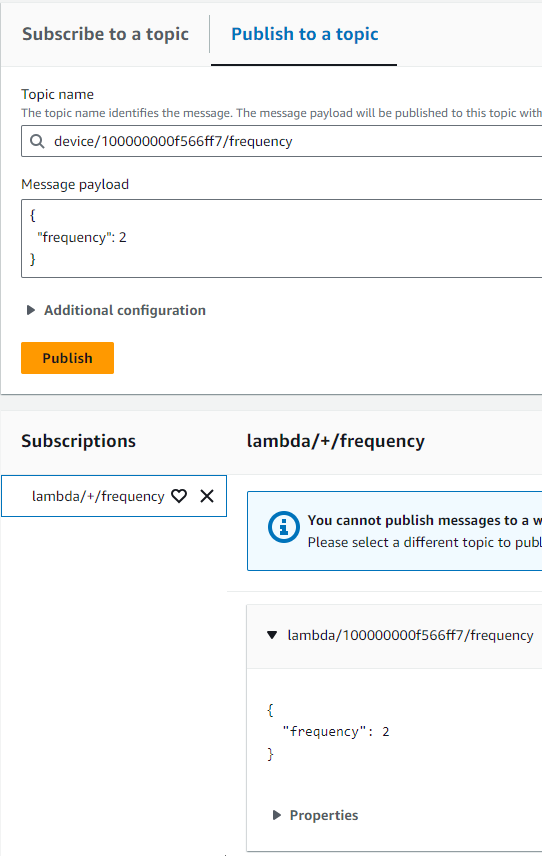
\includegraphics[width=.5\columnwidth]{validation/12_FrequencyChange.png}
    \captionof{figure}{Frequency change on \gls{aws}}
    \label{fig:12_FrequencyChange}
    \endgroup
\end{center}
Figure \ref{fig:12_LedApp_Log} shows the led application output message thread. It is possible to view different frequencies received on the Raspberry Pi 4.
\begin{center}
    \begingroup
    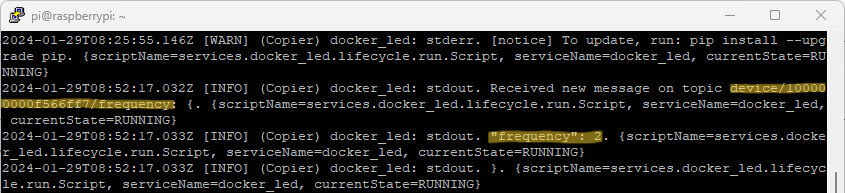
\includegraphics[width=1\columnwidth]{validation/12_LedApp_Log.png}
    \captionof{figure}{Frequency change on the Raspberry Pi 4}
    \label{fig:12_LedApp_Log}
    \endgroup
\end{center}
The button application was also tested. The external button on the Raspberry Pi 4 was pressed twice. \acrshort{mqtt} messages were transmitted to the led application locally and then published to \gls{aws} \acrshort{iot}. The messages can be seen in figure \ref{fig:12_ButtonChange}. The first press deactivates the blinking of the led and the second reactivates it.
\begin{center}
    \begingroup
    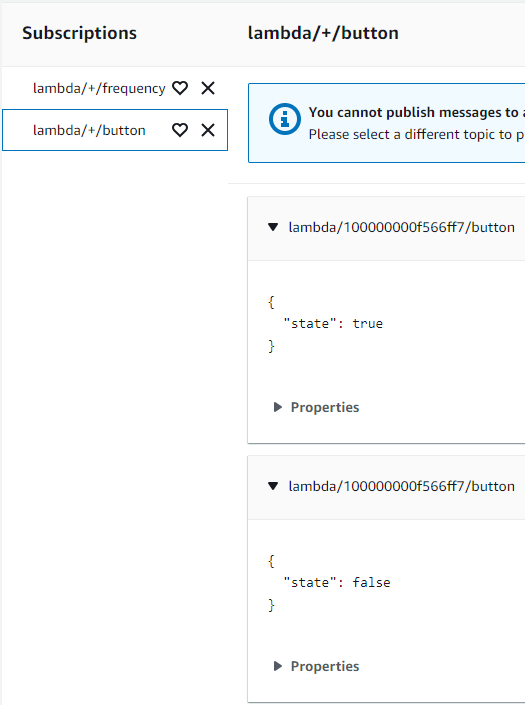
\includegraphics[width=.5\columnwidth]{validation/12_ButtonChange.png}
    \captionof{figure}{Blink status changes on \gls{aws}}
    \label{fig:12_ButtonChange}
    \endgroup
\end{center}
Figure \ref{fig:12_LedApp_Log_button} shows the output message thread of the led application. It is possible to view the \acrshort{mqtt} messages received from the button application on the Raspberry Pi 4.
\begin{center}
    \begingroup
    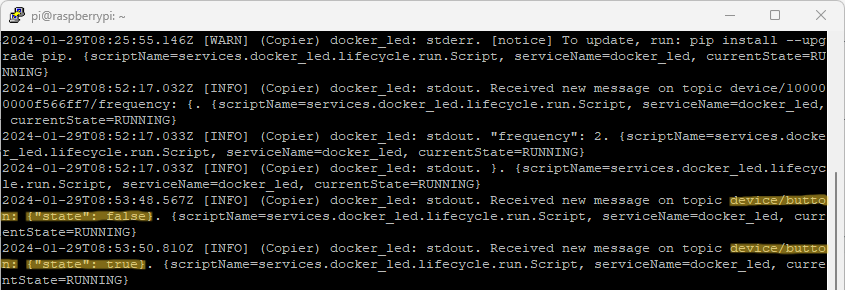
\includegraphics[width=1\columnwidth]{validation/12_LedApp_Log_button.png}
    \captionof{figure}{Blink status changes on the Raspberry Pi 4}
    \label{fig:12_LedApp_Log_button}
    \endgroup
\end{center}
Finally, the certificate was rotated. The triggering of a change alert was simulated from the \gls{aws} \acrshort{mqtt} interface by requesting the creation of \acrshort{csr} on the Raspberry Pi 4. Several \acrshort{mqtt} messages were exchanged. These are partly visible from the \gls{aws} interface in figure \ref{fig:12_CertRotate}. When analysing the digital twin, the certificate identifier was changed, proving that the rotation had indeed taken place. The Greengrass service was also restarted to take the new certificate into account.
\begin{center}
    \begingroup
    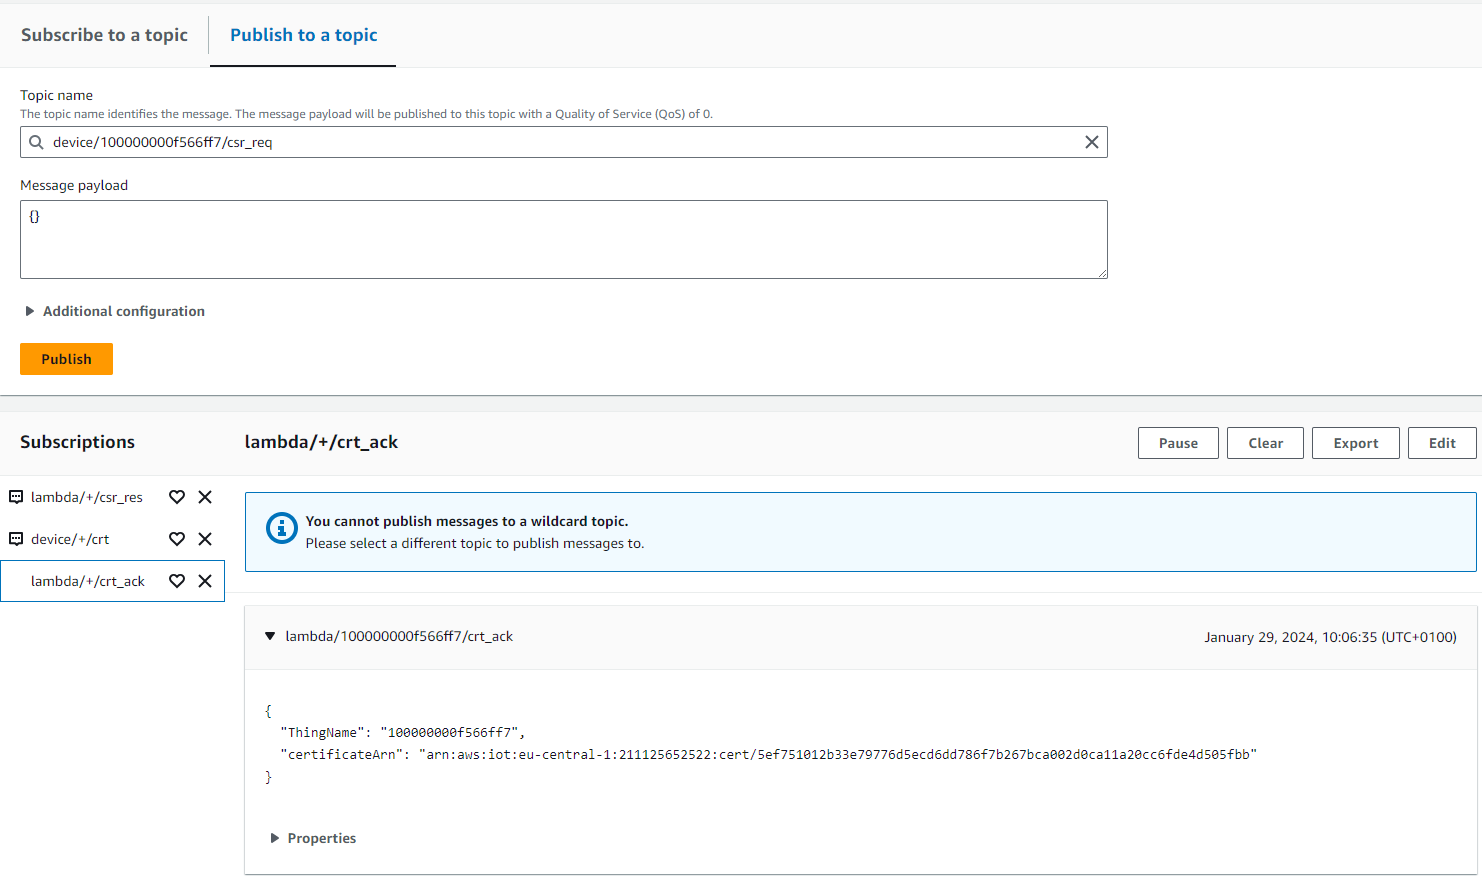
\includegraphics[width=1\columnwidth]{validation/12_CertRotate.png}
    \captionof{figure}{Certificate rotation on \gls{aws}}
    \label{fig:12_CertRotate}
    \endgroup
\end{center}
Figure \ref{fig:12_CertRotate_Log} shows the output message thread of the certificate rotation application. It is possible to view the \acrshort{mqtt} messages received from \gls{aws}. A request for \acrshort{csr} has been received as well as the new certificate.
\begin{center}
    \begingroup
    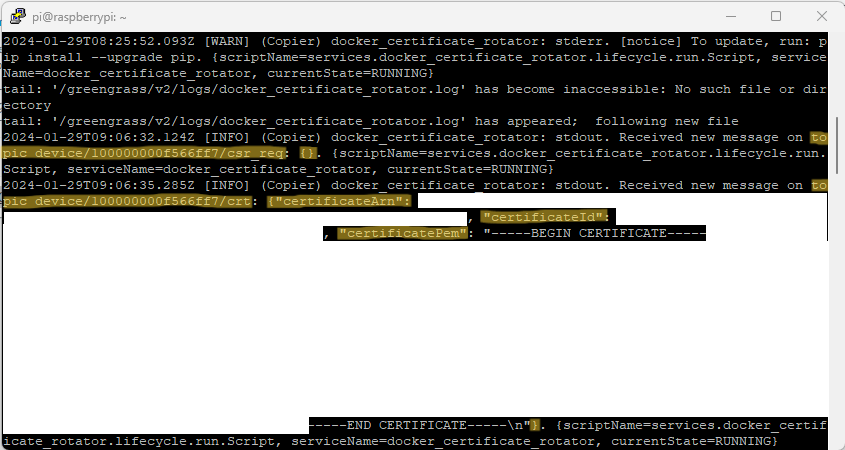
\includegraphics[width=1\columnwidth]{validation/12_CertRotate_Log.png}
    \captionof{figure}{Certificate rotation on the Raspberry Pi 4}
    \label{fig:12_CertRotate_Log}
    \endgroup
\end{center}

\subsection{Updating a component}

\section{\texorpdfstring{\Gls{cloud_infrastructure}}{} destruction}

% -- Your text goes here --

\section{Management of authorised embedded systems}

% -- Your text goes here --
\subsection{Infrastructure deployment with a provisioned embedded system}

\subsection{Unauthorised provisioning of an embedded system}

\subsection{Deleting a provisioned embedded system}

\section{Provisioning of other Arm SystemReady certified embedded systems}

% -- Your text goes here --

\section{\texorpdfstring{\Gls{cloud_infrastructure}}{} cost}

% -- Your text goes here --